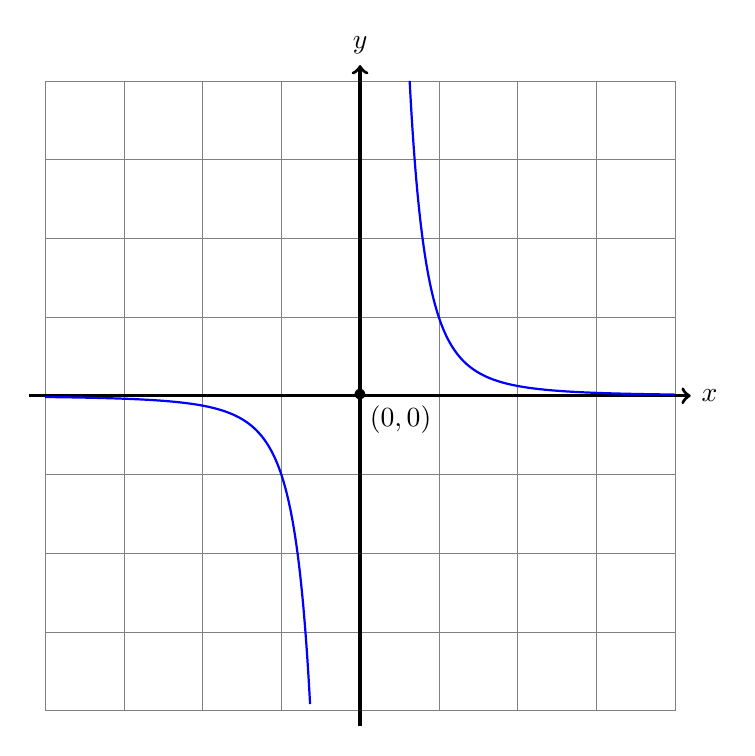
\begin{tikzpicture}
  \draw[very thin,color=gray] (-4,-4) grid (4,4);

  \draw[very thick,->] (-4.2,0) -- (4.2,0) node[right] {$x$};
  \draw[very thick,->] (0,-4.2) -- (0,4.2) node[above] {$y$};
  
  \draw [color=blue,thick] plot[smooth,samples=500,domain={(1/4)^(1/3)}:4] (\x,{(1/\x)^3});
  \draw [color=blue,thick] plot[smooth,samples=500,domain=-4:{-(1/4)^(1/3)}] (\x,{(1/\x)^3});

  \node at (0,0) {$\bullet$};
  \node [below right] at (0,0) {$(0,0)$};
\end{tikzpicture}
